\chapter{Herramientas utilizadas}
\label{cap:herramientas}

Este capítulo tiene por objetivo presentar y describir las herramientas computacionales utilizadas a lo largo de este trabajo. Específicamente, se abordará el programa \texttt{OpenMC}, los formatos de archivos usados (\texttt{MCPL} y \texttt{XML}), y los lenguajes de programación involucrados (\texttt{Python}, \texttt{C} y \texttt{C++}).

\section{\texttt{OpenMC}}

\texttt{OpenMC} es un programa de simulación Monte Carlo desarrollado inicialmente en el \textit{Massachusetts Institute of Technology} como \textit{software} de código abierto \cite{OpenMC2024}. Actualmente es mantenido por el \textit{Argonne National Laboratory} junto a una activa comunidad internacional que contribuye continuamente a su desarrollo y expansión. Está especialmente orientado al cálculo del transporte de neutrones y fotones, permitiendo tanto simulaciones de criticidad como simulaciones de fuente fija. En este trabajo se emplean exclusivamente simulaciones de fuente fija.

Una de las ventajas de \texttt{OpenMC} es su flexibilidad en la obtención de resultados. El código permite registrar diferentes magnitudes físicas como flujos, dosis, corrientes, espectros energéticos, etc., además de ofrecer la posibilidad de registrar partículas que atraviesan superficies definidas por quien utiliza el programa en un archivo de formato \texttt{HDF5} \cite{HDF5_2025} o \texttt{MCPL} \cite{MCPL2024}. Estos archivos almacenan información de las variables de las partículas, permitiendo su posterior análisis o reutilización para generar nuevas simulaciones. Asimismo, \texttt{OpenMC} incorpora técnicas avanzadas de reducción de varianza, como las ventanas de peso (\textit{weight windows}), que resultan fundamentales para reducir la incertidumbre estadística de los resultados en áreas de interés específico, técnica utilizada en este trabajo.

\section{\texttt{KDSource}}



\texttt{KDSource} es una herramienta computacional desarrollada en conjunto por CNEA e IB, cuyo objetivo principal es procesar archivos de partículas generados en simulaciones Monte Carlo para la construcción de nuevas fuentes distribucionales \cite{KDSource2024}. Su integración con \texttt{OpenMC} permite desacoplar geométricamente simulaciones complejas, facilitando significativamente el cálculo de transporte en geometrías difíciles o extensas.

El fundamento original de \texttt{KDSource} reside en la técnica \textbf{Kernel Density Estimation (KDE)}, una técnica estadística que permite estimar distribuciones continuas de variables a partir de muestras discretas, manteniendo la correlación existente entre ellas. 

\section{Formatos de listas de partículas: \texttt{MCPL} y \texttt{HDF5}}

En simulaciones Monte Carlo, es común registrar partículas que atraviesan una superficie o ingresan a una región de interés, generando lo que se conoce como una lista de partículas. Estos archivos permiten capturar el estado de cada partícula —incluyendo su energía, posición, dirección, peso estadístico y tipo de partícula— al momento de cruzar una superficie.

\texttt{OpenMC} emplea por defecto el formato \texttt{HDF5} para almacenar estas listas \cite{HDF5_2025}. Este formato binario jerárquico permite almacenar datos de manera eficiente, estructurada y accesible desde diversos lenguajes de programación. Sin embargo, su estructura está adaptada específicamente al ecosistema de \texttt{OpenMC}, dificultando su reutilización directa en otros códigos de transporte.

Con el objetivo de facilitar la interoperabilidad entre distintos códigos Monte Carlo, existe el formato \textbf{\texttt{MCPL} (\textit{Monte Carlo Particle List})} \cite{MCPL2024}. Este estándar de listas de partículas permite almacenar listas generadas en simulaciones de forma compacta y eficiente, preservando información esencial como la energía, posición, dirección, peso de cada partícula y tipo de partícula. A diferencia de formatos específicos como \texttt{HDF5}, \texttt{MCPL} fue concebido como una interfaz  entre diferentes entornos Monte Carlo.

La Figura \ref{fig:mcpl_support_diagram} muestra los diversos códigos que pueden producir o consumir archivos en formato \texttt{MCPL}. En este proyecto, su uso permite vincular eficientemente los archivos de partículas generados por \texttt{OpenMC} con la herramienta \texttt{KDSource}.

\section{Formato \texttt{XML}}

El formato \textbf{\texttt{XML} (\textit{Extensible Markup Language})} es un lenguaje utilizado para describir y almacenar información estructurada de manera jerárquica, basándose en una organización de datos tipo árbol \cite{XML2025}. Una de sus principales ventajas es que está diseñado para ser tanto legible por máquinas como por humanos, lo que facilita su edición, inspección y validación manual durante el desarrollo. Debido a estas características, resulta particularmente adecuado para guardar las distribuciones estimadas mediante histogramas multidimensionales. A su vez, \texttt{OpenMC} emplea archivos \texttt{XML} para almacenar la configuración completa de sus simulaciones (geometría, materiales, configuración de \textit{tallies}, etc.), por lo que la elección de este formato contribuye a una integración directa y eficiente entre los componentes desarrollados.

\begin{figure}[H]
    \centering
    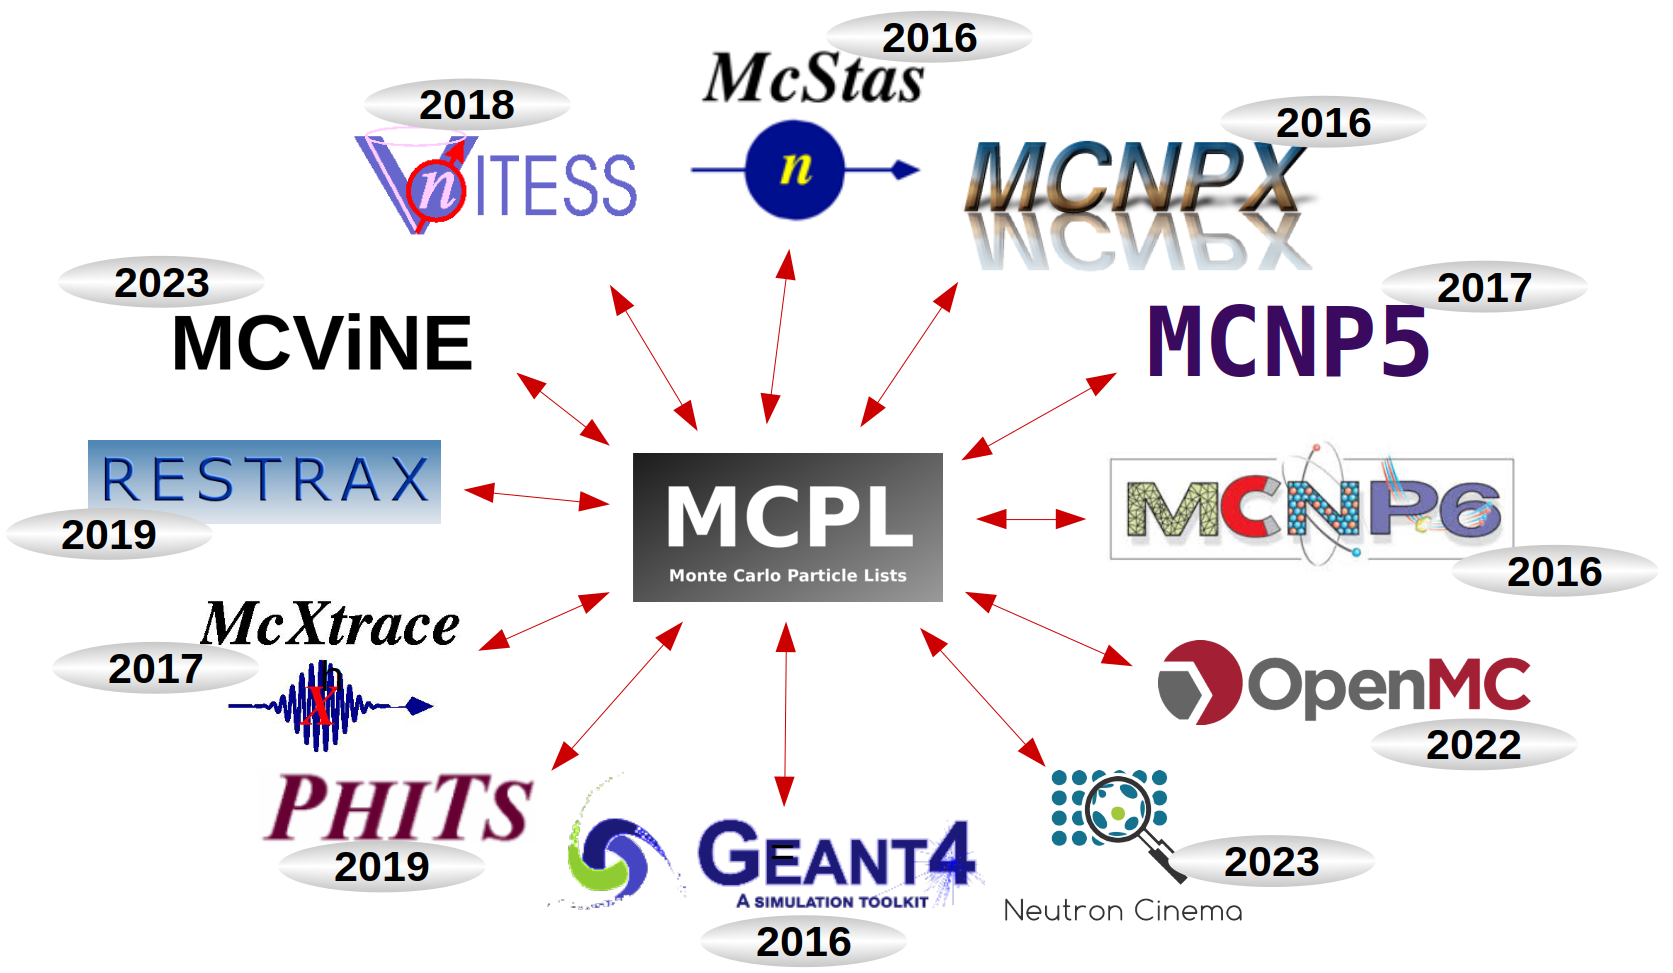
\includegraphics[width=\textwidth]{figs/mcpl_support_diagram.png}
    \caption[Diagrama de soporte de \texttt{MCPL}.]{Diagrama de soporte de \texttt{MCPL}. Reproducido de \cite{MCPL2024}.}
    \label{fig:mcpl_support_diagram}
\end{figure}

\section{Lenguajes de programación: \texttt{Python}, \texttt{C} y \texttt{C++}}

A lo largo del desarrollo del proyecto, se utilizaron principalmente tres lenguajes de programación:

\begin{itemize}
    \item \textbf{\texttt{Python}}: lenguaje de alto nivel especialmente adecuado para interfaces de usuario, análisis exploratorio de datos y configuración de simulaciones debido a su simplicidad, claridad y flexibilidad. \texttt{KDSource} hace uso de \texttt{Python} para la preparación y procesamiento de datos previos al remuestreo Monte Carlo. Tanto \texttt{KDSource} como \texttt{OpenMC} disponen de una interfaz en Python.

    \item \textbf{\texttt{C}}: lenguaje de programación de bajo nivel conocido por su eficiencia computacional, velocidad y control preciso sobre la gestión de memoria. Se utilizó en este trabajo para desarrollar módulos específicos encargados del remuestreo eficiente de partículas, especialmente cuando se requieren grandes volúmenes de datos. El módulo de remuestreo de \texttt{KDSource} está escrito en este lenguaje.
    
    \item \textbf{\texttt{C++}}: lenguaje de programación que extiende a \texttt{C} con capacidades de programación orientada a objetos. Esta arquitectura permite la expansión modular del código y facilita su mantenimiento. \texttt{OpenMC} está desarrollado en este lenguaje.


\end{itemize}


El desarrollo realizado en este trabajo implementa un flujo computacional para el uso de fuentes distribucionales en simulaciones Monte Carlo. Este flujo se compone de tres etapas principales: detección, procesamiento y producción, y aprovecha las capacidades de los lenguajes \texttt{Python}, \texttt{C} y \texttt{C++}.

\textbf{Detección}: se realiza mediante una simulación inicial en \texttt{OpenMC}, en la cual se registra un archivo de partículas sobre una superficie. Este archivo puede guardarse en formato \texttt{HDF5}, que es el formato nativo de \texttt{OpenMC}, y luego ser convertido al formato \texttt{MCPL} si se desea continuar con el procesamiento. Alternativamente, si \texttt{OpenMC} fue compilado con soporte para \texttt{MCPL}, puede generarse directamente en dicho formato. El archivo resultante se almacena en disco para su uso posterior. Este procedimiento se ilustra en la Figura \ref{fig:flujo_deteccion}.

\begin{figure}[H]
    \centering
    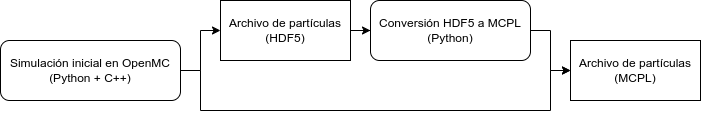
\includegraphics[width=0.75\textwidth]{flujo_codigos-Deteccion.png}
    \caption{Etapa de detección: registro de partículas en formato \texttt{MCPL} a partir de una simulación en \texttt{OpenMC}. Bloques con esquinas redondeadas representan procesos computacionales, mientras que los bloques rectangulares indican archivos que se registran o leen desde disco.}
    \label{fig:flujo_deteccion}
\end{figure}

\textbf{Procesamiento}: esta etapa se lleva a cabo en \texttt{Python} utilizando la implementación desarrollada para procesar mediante histogramas multidimensionales. A partir del archivo \texttt{MCPL}, se construye una fuente distribucional que representa la densidad de probabilidad estimada en el espacio de fases. El resultado de esta etapa es un archivo \texttt{XML}, que contiene la parametrización de la fuente y se almacena en disco como entrada para la etapa de producción. Este archivo \texttt{XML} constituye toda la información necesaria para generar nuevas partículas en simulaciones posteriores, sin requerir el acceso al archivo original de partículas. Esta característica representa una ventaja frente al método utilizado en \texttt{KDSource}, el cual necesita mantener el archivo original disponible en memoria durante la simulación posterior. Sin embargo, ambos métodos necesitan cargar en memoria el archivo de partículas original para el procesamiento. En casos donde dicho archivo posea un volumen considerable pueden derivar en un consumo elevado de memoria \textit{RAM}. La Figura \ref{fig:flujo_procesamiento} muestra un esquema de esta etapa.

\begin{figure}[H]
    \centering
    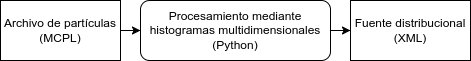
\includegraphics[width=0.55\textwidth]{flujo_codigos-Procesamiento.png}
    \caption{Etapa de procesamiento: construcción de una fuente distribucional a partir de un archivo \texttt{MCPL}. Bloques con esquinas redondeadas representan procesos computacionales, mientras que los bloques rectangulares indican archivos que se registran o leen desde disco.}
    \label{fig:flujo_procesamiento}
\end{figure}

\textbf{Producción}: esta etapa puede abordarse de dos maneras, implementada en código \texttt{C}. En la modalidad \textit{offline}, el archivo \texttt{XML} es utilizado para generar una nueva lista de partículas en formato \texttt{MCPL}, que luego puede emplearse directamente como fuente en \texttt{OpenMC} si se cuenta con soporte para este formato. En caso contrario, puede convertirse nuevamente a \texttt{HDF5}. En la modalidad \textit{on-the-fly}, se evita por completo el uso de listas intermedias: \texttt{OpenMC} accede directamente al archivo \texttt{XML} y realiza el remuestreo dinámicamente durante la simulación, gracias a una extensión \emph{ad-hoc} incorporada en este trabajo. Ambas modalidades se ilustran en la Figura \ref{fig:flujo_produccion}.

\begin{figure}[H]
    \centering
    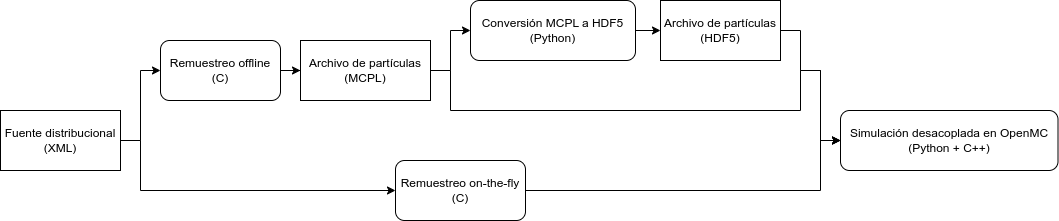
\includegraphics[width=\textwidth]{flujo_codigos-Remuestreo.png}
    \caption{Etapa de producción: uso del archivo \texttt{XML} para generar nuevas partículas de forma offline o on-the-fly. Bloques con esquinas redondeadas representan procesos computacionales, mientras que los bloques rectangulares indican archivos que se registran o leen desde disco.}
    \label{fig:flujo_produccion}
\end{figure}



